\documentclass{standalone}
\usepackage[T1]{fontenc}
\usepackage[latin2]{inputenc}
\usepackage[english]{babel}
\usepackage{tikz}
\usepackage{times}
\usetikzlibrary{calc,through,backgrounds,positioning,fit}
\usetikzlibrary{shapes,arrows,shadows}
 
\begin{document}
 
 
\centering
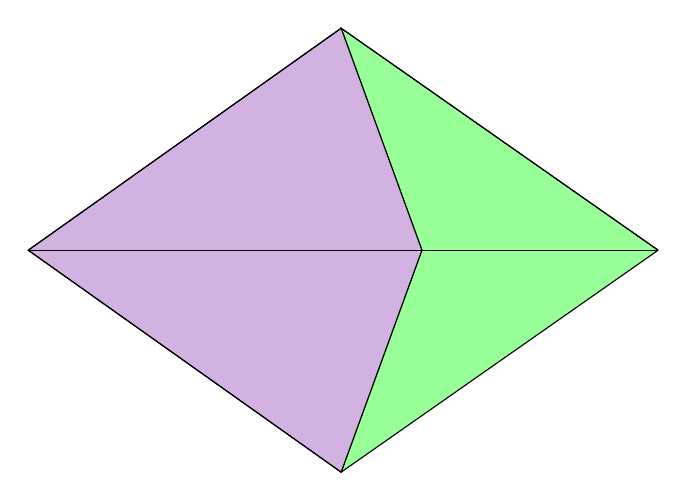
\begin{tikzpicture}

\draw (0,0) -- (0:3) coordinate (p1);
\draw (0,0) -- (110:3) coordinate (p2);
\draw (0,0) -- (180:5) coordinate (p3);
\draw (0,0) -- (250:3) coordinate (p4);
\fill[green!40, draw=black](p1) -- (p2) -- (0,0)--(p4);
\fill[blue!60!red!30!, draw=black](p2) -- (p3) -- (p4)--(0,0)--(p2);
\draw (0,0) -- (p1);
\draw (0,0) -- (p3);
\draw (p1) -- (p2) --(p3)--(p4)--(p1);

\end{tikzpicture}

 
\end{document}